\documentclass{article}
\usepackage{tikz}
\usepackage{float} 
\usepackage{algorithm}
\usepackage{algpseudocode}
\usepackage{amsmath}
\usepackage{amssymb}
\usepackage{amsthm}
\usepackage{placeins}
\usepackage{hyperref}

% Define the 'definition' environment
\newtheorem{definition}{Definition}

\title{Segment Trees in Algorithmic Problems}
\author{Piotr Szczepaniak}
\date{\today}

\begin{document}

\maketitle

\tableofcontents

\begin{abstract}
This document provides an overview of segment trees. In the first place
I will describe some basic implementation and use case for segment trees.
Then we will try to understand the algebraic properties of segment trees for
better understanding of how they work. Finally we will dive in some more complex and not so obvious
use cases of segment trees.
\end{abstract}

\section{Foundations of Segment Trees}
Basic use case of segment tree is to store information about segments of an array.
Consider an array \(A\) with some data stored in it. To be able to perform operations on segments of this array, like
give the max value in \(A[i, j]\) or give the sum of elements in \(A[i, j]\), we can use a segment tree for faster
access answers to these queries. Additionally segment tree allows us to update values in the array and still be able to perform queries on segments quickly.
A segment tree is a binary tree used for storing information about segments with quick acces to the data stored in it. 
To efficently retrieve or update informations about elements stored 
in segment tree we can perform various operations most common of which are
query/update on point or range.
One of the examples can be maximum value of 
elements in given range or sum of elements in given range.

\begin{figure}[H]
    \centering
    
\begin{center}
    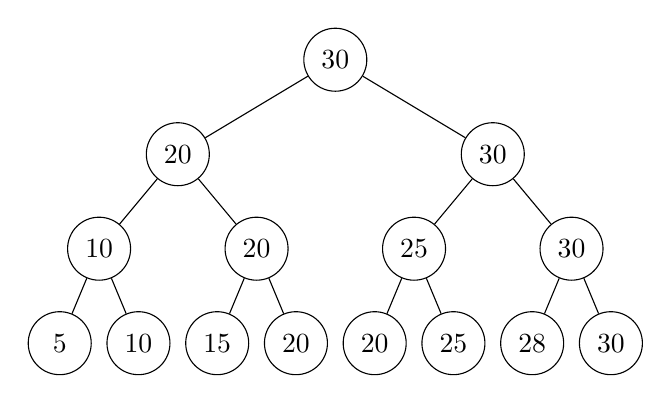
\begin{tikzpicture}[
      level distance=1.2cm,
      level 1/.style={sibling distance=4cm},
      level 2/.style={sibling distance=2cm},
      level 3/.style={sibling distance=1cm},
      every node/.style={draw,circle,minimum size=8mm,inner sep=1pt}
    ]
    
    % Root node with max value
    \node {30}
        child {node {20}
            child {node {10}
                child {node {5}}
                child {node {10}}
            }
            child {node {20}
                child {node {15}}
                child {node {20}}
            }
        }
        child {node {30}
            child {node {25}
                child {node {20}}
                child {node {25}}
            }
            child {node {30}
                child {node {28}}
                child {node {30}}
            }
        };
    
    \end{tikzpicture}
\end{center}
    \caption{Example of a segment tree with maximum value of elements in given range.}
    \label{fig:segment_tree_1}
\end{figure}

\subsection{Segment Tree with point update and range query}
To ilustrate use case of segment tree we will construct tree with max value on segment.
Let's say we are given an array \(A = [5, 10, 15, 20, 30, 25, 28, 20]\) of length \(n = 8\).
For now let's assume that the input array is of size \(n = 2^{k}\) where \(k\) is integer (for different
sizes of input we will fill input array with neutral elements (see section 2) to make it's length a power of 2).
In the following implementation a segment tree is acctually an array of size \(2n - 1\) where we store the whole structure.
The leaves of the tree will store the values of the array and the internal nodes will store the maximum value of the elements in their subtree.
For every internal node \(i\) the children of this node will be \(2i\) and \(2i + 1\), and the root of the tree will be at index 1.
We want to be able to perform the following operations:
\begin{itemize}
    \item \textbf{Build structure} \\
    We will create a segment tree from an array.
    To build a segment tree, we need to create a binary tree where each node will store the maximum value of elements in its subtree.
    First we copy elements of array to the leaves of the tree (as \(max(A[i, i]) = A[i]\)), then we build the tree from bottom to the top \\
    \begin{algorithm}
    \caption{Build Segment Tree for Maximum on Segment (Iterative)}
    \begin{algorithmic}
        \Procedure{BuildTree}{arr, seg}
            \For{$i = 0$ \textbf{to} $n - 1$} \Comment{Fill leaves of the segment tree}
                \State $seg[n + i] \gets A[i]$
            \EndFor
            \For{$i = n - 1$ \textbf{downto} $1$} \Comment{Calculates nodes from bottom to top}
                \State $seg[i] \gets \max(seg[2 \times i], seg[2 \times i + 1])$
            \EndFor
        \EndProcedure
    \end{algorithmic}
\end{algorithm}
    \FloatBarrier
    \item \textbf{Point update} \\
    Now let's update single value in the array and update the tree.
    We will change the value of \(A[1]\) from 10 to 35.
    To update the tree we need to change the value of the leaf node 
    and then update all the parent nodes up to the root.
    \begin{algorithm}
    \caption{Point Update on Segment Tree }
    \begin{algorithmic}
        \Procedure{update}{seg, index, value}
            \State $index \gets index + n$ \Comment{Shift index to leaf}
            \State $arr[index] \gets value$ \Comment{Update the value at the leaf}
            \While{$index > 1$} \Comment{Update the parent nodes}
                \State $index \gets \lfloor index / 2 \rfloor$
                \State $arr[index] \gets \max(arr[2 \times index], arr[2 \times index + 1])$
            \EndWhile
        \EndProcedure
    \end{algorithmic}
\end{algorithm}
    \begin{figure}[H]
        \centering
        
\begin{center}
    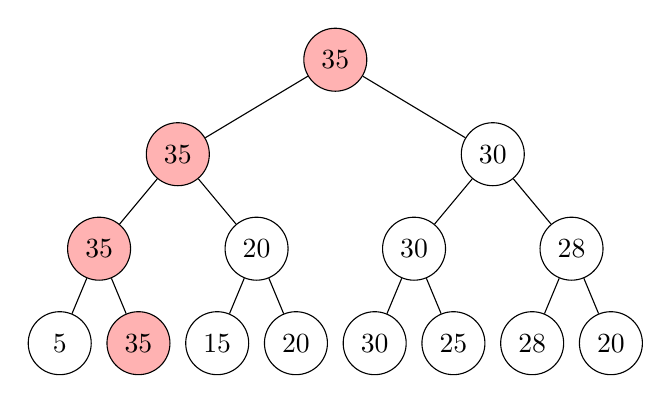
\begin{tikzpicture}[
      level distance=1.2cm,
      level 1/.style={sibling distance=4cm},
      level 2/.style={sibling distance=2cm},
      level 3/.style={sibling distance=1cm},
      every node/.style={draw,circle,minimum size=8mm,inner sep=1pt}
    ]
    
    % Root node with max value
    \node[fill=red!30] {35}
        child {node[fill=red!30] {35}
            child {node[fill=red!30] {35}
                child {node {5}}
                child {node[fill=red!30] {35}}
            }
            child {node {20}
                child {node {15}}
                child {node {20}}
            }
        }
        child {node {30}
            child {node {30}
                child {node {30}}
                child {node {25}}
            }
            child {node {28}
                child {node {28}}
                child {node {20}}
            }
        };
    
    \end{tikzpicture}
\end{center}

        \caption{Example of point update.}
        \label{fig:segment_tree_2}
    \end{figure}

    \item \textbf{Range query} \\
    Now let's say we want to find the maximum value in the range \(A[3:8]\).
    To do this we need to traverse the tree from the root to the leaves and 
    find nodes that are in the range (which means that every leaf in the subtree of this node is in the range of the query). 
    Then we will get max the values of these nodes to get the final result.
    To get the result for range \(A[3:8]\) we call \(RangeQuery(seg, 1, 1, 9, 3, 9)\).

    \begin{algorithm}
    \caption{Range Maximum Query on Segment Tree (Recursive, Close-Open Range)}
    \begin{algorithmic}[1]
        \Procedure{RangeQuery}{seg, index, l, r, a, b}
            \Comment{index: current node index in seg}
            \Comment{[l, r): segment represented by current node}
            \Comment{[a, b): query range}
            \If{$b \le l$ \textbf{or} $r \le a$}
                \State \Return $-\infty$ \Comment{No overlap}
            \ElsIf{$a \le l$ \textbf{and} $r \le b$}
                \State \Return $seg[index]$ \Comment{Total overlap}
            \Else
                \State $mid \gets \left\lfloor \frac{l + r}{2} \right\rfloor$
                \State $left \gets$ \Call{RangeQuery}{seg, $2 \cdot index$, $l$, $mid$, $a$, $b$}
                \State $right \gets$ \Call{RangeQuery}{seg, $2 \cdot index + 1$, $mid$, $r$, $a$, $b$}
                \State \Return $\max(left, right)$
            \EndIf
        \EndProcedure
    \end{algorithmic}
\end{algorithm}

    \begin{figure}[H]
        \centering
        
\begin{center}
    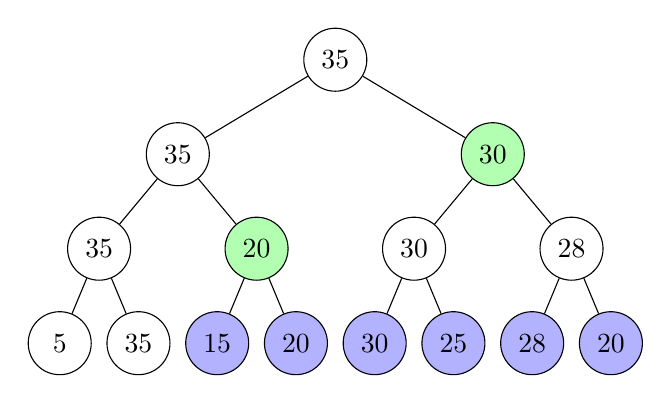
\begin{tikzpicture}[
      level distance=1.2cm,
      level 1/.style={sibling distance=4cm},
      level 2/.style={sibling distance=2cm},
      level 3/.style={sibling distance=1cm},
      every node/.style={draw,circle,minimum size=8mm,inner sep=1pt}
    ]
    
    % Root node with max value
    \node {35}
        child {node {35}
            child {node {35}
                child {node {5}}
                child {node {35}}
            }
            child {node[fill=green!30] {20}
                child {node[fill=blue!30]  {15}}
                child {node[fill=blue!30]  {20}}
            }
        }
        child {node[fill=green!30]  {30}
            child {node {30}
                child {node[fill=blue!30]  {30}}
                child {node[fill=blue!30]  {25}}
            }
            child {node  {28}
                child {node[fill=blue!30]  {28}}
                child {node[fill=blue!30] {20}}
            }
        };
    
    \end{tikzpicture}
\end{center}

        \caption{Example of range query. Blue leafs represents subarray \(A[2:7]\). Green nodes 
        are the nodes that totally overlap, red ones that don't overlap and yellow ones that partially overlap (are called in recursion).}
        \label{fig:segment_tree_3}
    \end{figure}

\end{itemize}

\subsection{Segment Tree with range update and point query}
This type of segment tree is very similar to previous one but in this case we will be able
to perform updates on given range and ask what is the value of an array at given index.
The difference from the previous example is taht in the nodes of the tree don't keep the
actual values of the array but some value that modifies the value from array. 
Let's take example were we add value to all elements of array on the given range. 
If the node has value $x$ it means that we added $x$ to all elements in the range of this node.
So in order to get the value of the array at given index we need to traverse the tree 
from the leaf to the root and sum all values of the nodes we passed.

\begin{itemize}
    \item \textbf{Build structure} \\
    To create a tree we only copy elements of the array to the leaves of the tree, 
    because there are no updates yet.
    \FloatBarrier
    \item \textbf{range update} \\
    Here we want to add some given value $x$ to all elements in the range $A[a:b]$.
    This operation is similar to the range query from previous tree but here instead of
    returning the maximum value we will update the value of the node.
    \begin{algorithm}
    \caption{Range Update on Segment Tree (Recursive, Close-Open Range)}
    \begin{algorithmic}[1]
        \Procedure{RangeQuery}{seg, index, l, r, a, b, x}
            \If{$b \leq l$ \textbf{or} $r \leq a$}
                \State \Return
            \ElsIf{$a \leq l$ \textbf{and} $r \leq b$}
                \State $seg[index] \gets seg[index] + x$
            \Else
                \State $mid \gets \left\lfloor \frac{l + r}{2} \right\rfloor$
                \State \Call{RangeQuery}{seg, $2 \cdot index$, $l$, $mid$, $a$, $b$, $x$}
                \State \Call{RangeQuery}{seg, $2 \cdot index + 1$, $mid$, $r$, $a$, $b$, $x$}
                \State \Return
            \EndIf
        \EndProcedure
    \end{algorithmic}
\end{algorithm}
    \begin{figure}[H]
        \centering
        
\begin{center}
    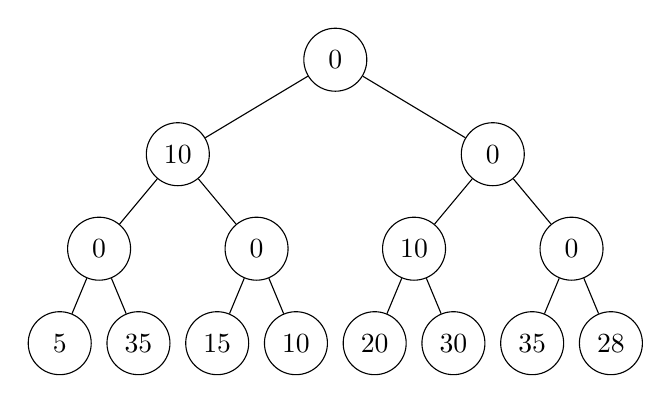
\begin{tikzpicture}[
      level distance=1.2cm,
      level 1/.style={sibling distance=4cm},
      level 2/.style={sibling distance=2cm},
      level 3/.style={sibling distance=1cm},
      every node/.style={draw,circle,minimum size=8mm,inner sep=1pt}
    ]
    
    % Root node with max value
    \node {0}
        child {node {10}
            child {node {0}
                child {node {5}}
                child {node {35}}
            }
            child {node {0}
                child {node {15}}
                child {node {10}}
            }
        }
        child {node {0}
            child {node {10}
                child {node {20}}
                child {node {30}}
            }
            child {node {0}
                child {node {35}}
                child {node {28}}
            }
        };
    
    \end{tikzpicture}
\end{center}

        \caption{Example of range update. This is a state of the tree for initial array $A = [5, 35, 15, 10, 20, 30, 25, 28]$ after range update on range $A[0:6]$ by adding value 10.}
    \end{figure}

    \item \textbf{point query} \\
    Let's think about what we keep in the nodes of the tree, and how to retrieve the value of the array at given index $i$.
    When we made some update within the range of $i$ we added some value in the node that is on the path from the leaf to the root.
    Even leaf node is actually a modifier applied to neutral element 0. The result of the query is the sum of all values in the nodes on the path from the leaf to the root.
    That is a value of all modifiers on the path that were applied to the neutral element 0.
    Here we use iterative approach as recursive one would be too complex and not very efficient.
    \begin{algorithm}
    \caption{Point Query on Segment Tree }
    \begin{algorithmic}
        \Procedure{query}{seg, index}
            \State $index \gets index + n$ \Comment{Shift index to leaf}
            \State $result \gets 0$ \Comment{Initialize result with the neutral value}
            \While{$index \geq 1$} 
                \State $result \gets result + arr[index]$
                \State $index \gets \lfloor index / 2 \rfloor$
            \EndWhile
        \EndProcedure
    \end{algorithmic}
\end{algorithm}

    If we for example ask for the value at index 0 of the array after the update visualized in
    the tree above, we will get the value 15. \\
    \textit{Note: What would happend if we instead of adding the value to the nodes we would 
    set the value of the nodes in the range? Would this tree still work? No.
    This operation is not commutative and the result of the query would depend on the order of the updates.
    To sole problem like this we need to use \textbf{lazy propagation} which is a more complex version of segment tree.}
\end{itemize}

\subsection{Segment Tree with range update and range query}
A Little more complex version of segment tree is a segment tree with range update and range query which require \textbf{lazy propagation}.
We will consider a segment tree with sum of elements in given range. 
Apart form values in tree we will also store lazy values in each node.
The lazy value is used to delay the update of a node until it is needed, and 
to solve problem of non-commutative updates.


\begin{itemize}
    \item \textbf{Build structure} 
    Only difference form previus example is initializig the lazy value for all nodes \\
    \begin{algorithm}
    \caption{Build Segment Tree for Sum on Segment (Iterative)}
    \begin{algorithmic}
        \Procedure{BuildTree}{arr, seg}
            \For{$i = 0$ \textbf{to} $n - 1$} \Comment{Fill leaves of the segment tree}
                \State $seg[n + i] \gets \{A[i], 0\}$ \Comment{second value is for lazy propagation}
            \EndFor
            \For{$i = n - 1$ \textbf{downto} $1$} \Comment{Calculates nodes from bottom to top}
                \State $seg[i] \gets \{\max(seg[2 \times i], seg[2 \times i + 1]), 0\}$
            \EndFor
        \EndProcedure
    \end{algorithmic}
\end{algorithm}\\


    \item \textbf{Range update} \\
    In this case lazy value is a value that we want to add to all elements in the range.
    Another way to think about this is that we want to add lazy value to all elenets in arrary 
    which are represented by all leaves in subtree of given node.
    \begin{algorithm}
    \caption{Range Update on Segment Tree }
    \begin{algorithmic}
        \Procedure{QueryUpdate}{seg, lazy index, l, r, a, b, value} \Comment{Value: value we wanted to add to each element in array}
            \State $size = r - l + 1$
            \If{$b < l$ \textbf{or} $a > r$}
                \State \Return
            \ElsIf{$a \leq l$ \textbf{and} $r \leq b$}
                \State $seg[index] \gets {seg[index] + value*size}$
                \State $lazy[index] \gets {lazy[index] + value}$
                \State \Return
            \Else
                \State $seg[index*2] \gets {seg[index*2] + value*size}$ \Comment{Update left child}
                \State $lazy[index*2] \gets {lazy[index*2] + value}$ \Comment{Push lazy to left child}
                \State $seg[index*2+1] \gets {seg[index*2+1] + value*size}$ \Comment{Same to right}
                \State $lazy[index*2+1] \gets {lazy[index*2+1] + value}$ 
                \State $lazy[index] \gets {0}$ \Comment{Reset lazy value for current node}
                \State $mid \gets \left\lfloor \frac{l + r}{2} \right\rfloor$
                \State $left \gets$ \Call{QueryUpdate}{seg, $2 \cdot index$, $l$, $mid$, $a$, $b$, $value$}
                \State $right \gets$ \Call{QueryUpdate}{seg, $2 \cdot index + 1$, $mid + 1$, $r$, $a$, $b$, $value$}
                \State $seg[index] \gets {seg[index*2] + seg[index*2+1] + lazy[index]*size}$ \Comment{Update current node after lazy propagation}
            \EndIf
        \EndProcedure
    \end{algorithmic}
\end{algorithm} \\
    How this algorithm works:
    \begin{enumerate}
        \item If the current node is fully in range update the sum of the node and set the lazy value. Sum - $value*size$ where $size$ is the number of array elements (leafs) in the range of this node, Lazy is equal to $value$, which we will later push down to child nodes.
        \item Call the function recursively for the left and right child nodes.
        \item Finally update the sum of the current node with the sum of its children.
        \item Moving back to the top from recursion, we will update the sum of the current node with the sum of its children so that the value in the nodes above have correct value after update.
    \end{enumerate}
On the following example we will update the range \(A[0:5]\) by adding 10 to all elements in this range
where initial array is \(A = [5, 10, 15, 20, 30, 25, 20, 20]\).
    
    \begin{figure}[H]
        \centering
        
\begin{center}
    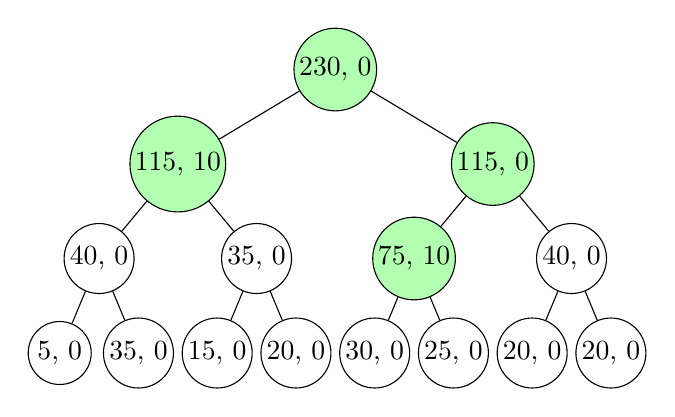
\begin{tikzpicture}[
      level distance=1.2cm,
      level 1/.style={sibling distance=4cm},
      level 2/.style={sibling distance=2cm},
      level 3/.style={sibling distance=1cm},
      every node/.style={draw,circle,minimum size=8mm,inner sep=1pt}
    ]
    
    % Root node with max value
    \node[fill=green!30] {230, 0}
        child {node[fill=green!30] {115, 10}
            child {node {40, 0}
                child {node {5, 0}}
                child {node {35, 0}}
            }
            child {node {35, 0}
                child {node  {15, 0}}
                child {node {20, 0}}
            }
        }
        child {node[fill=green!30] {115, 0}
            child {node[fill=green!30] {75, 10}
                child {node {30, 0}}
                child {node {25, 0}}
            }
            child {node  {40, 0}
                child {node {20, 0}}
                child {node {20, 0}}
            }
        };
    
    \end{tikzpicture}
\end{center}

        \caption{This is state of the tree after range update. Green nodes were changed during the update.}
        \label{fig:segment_tree_4}
    \end{figure}

    \item \textbf{Range query} 
    We will try to retrieve the sum of some given range. The algorithm for this will be simiar to the one for range update.
    First we will check if the current node is fully in range. If it is we add the sum of this node, propagating lazy values along the way.
    \begin{algorithm}[H]
    \caption{Range Query on Segment Tree for Max with Modifiers}
    \begin{algorithmic}
        \Procedure{RangeQuery}{seg, index, l, r, a, b}
            \If{$b \leq l$ \textbf{or} $r \leq a$}
                \State \Return $-\infty$
            \EndIf
            \If{$a \leq l$ \textbf{and} $r \leq b$}
                \State \Return $seg[index].val$
            \EndIf
            \State $mid \gets \left\lfloor \frac{l + r}{2} \right\rfloor$
            \State $left \gets$ \Call{RangeQuery}{seg, $2 \cdot index$, $l$, $mid$, $a$, $b$}
            \State $right \gets$ \Call{RangeQuery}{seg, $2 \cdot index + 1$, $mid$, $r$, $a$, $b$}
            \State \Return $\max(left, right) + seg[index].mod$
        \EndProcedure
    \end{algorithmic}
\end{algorithm}
 
    \begin{figure}[H]
        \centering
        
\begin{center}
    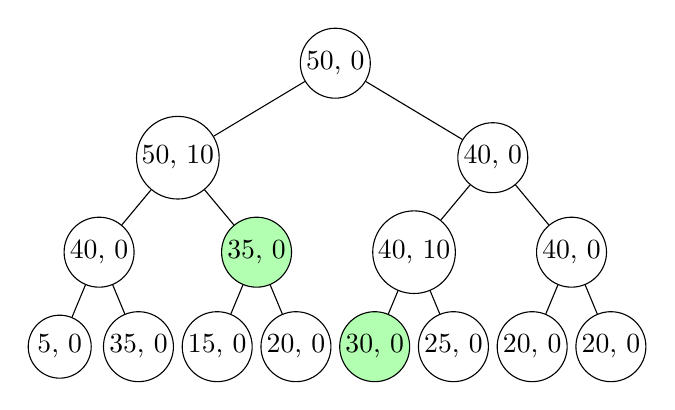
\begin{tikzpicture}[
      level distance=1.2cm,
      level 1/.style={sibling distance=4cm},
      level 2/.style={sibling distance=2cm},
      level 3/.style={sibling distance=1cm},
      every node/.style={draw,circle,minimum size=8mm,inner sep=1pt}
    ]
    
    % Root node with max value
    \node {50, 0}
        child {node {50, 10}
            child {node {40, 0}
                child {node {5, 0}}
                child {node {35, 0}}
            }
            child {node [fill=green!30] {35, 0}
                child {node  {15, 0}}
                child {node {20, 0}}
            }
        }
        child {node {40, 0}
            child {node {40, 10}
                child {node [fill=green!30] {30, 0}}
                child {node {25, 0}}
            }
            child {node  {40, 0}
                child {node {20, 0}}
                child {node {20, 0}}
            }
        };
    
    \end{tikzpicture}
\end{center}

        \caption{This is state of the tree after range query on range [2: 4]. Green nodes were we took values form to the sum. Result of query is 95.}
        \label{fig:segment_tree_5}
    \end{figure}

\end{itemize}


\section{A mathematical approach to segment trees}
In this section we will try to understand how segment trees work and why they are so efficient.
In order to do this we will need to understand some basic algebra that is used in segment trees.


\subsection{Monoids}
A monoid \( (S, \ast, e) \) is a set equipped with an associative binary operation \( S \times S \to S \) and
an identity element \(e\). 
\begin{itemize}
    \item \textbf{Associativity} \\
    For all \( a, b, c \in S \), \( (a \ast b) \ast c = a \ast (b \ast c) \).
    \item \textbf{Identity element} \\
    There exists an element \( e \in S \) such that for all \( a \in S \), \( a \ast e = e \ast a = a \).
    \item \textbf{Commutativity} \\
    Monoid is called \textbf{commutative} if for all \( a, b \in S \), \( a \ast b = b \ast a \).
\end{itemize}
Examples of monoids:
\begin{itemize}
    \item \textbf{Natural numbers under addition, (\(\mathbb{N}\), +, 0) } \\
    In this simple example we can see that addition is associative and commutative. 
    Adding 0 (neutral element) to any of the numbers will not change the result of the operation.
    \item \textbf{Strings over an alphabet, (\(\Sigma^*\), \(\cdot\), \(\epsilon\))} \\
    \(\Sigma^*\) - set of all strings over an alphabet \(\Sigma\) \\
    \(\cdot\) - concatenation of strings \\
    \(\epsilon\) - empty string \\
    This is a example of non-commutative monoid. Concatenation of strings is associative but not commutative as we can see in the following example.
    \begin{equation}
        \text{abc} \cdot \text{def} = \text{abcdef} \neq \text{defabc} = \text{def} \cdot \text{abc}
    \end{equation}
\end{itemize}
\subsection{Homomorphism}
A homomorphism is a structure-preserving map between two algebraic structures.
In this section we will look at homomorphisms between monoids.
Let \( (S, \ast, e) \) and \( (T, \cdot, \theta) \) be two monoids.
A function \( f: S \to T \) is a homomorphism if:
\begin{itemize}
    \item \textbf{Preserves the operation} \\
    For all \( a, b \in S \), \( f(a \ast b) = f(a) \cdot f(b) \).
\end{itemize}
Let's consider a simple example of homomorphism between two monoids.
Let \( S = (\mathbb{N}, +, 0) \) and \( T = (\mathbb{N}, \cdot, 1) \).
Let \( f: S \to T \) be defined as \( f(x) = 2^x \).
We can see that:
\begin{itemize}
    \item \( f(a + b) = 2^{a + b} = 2^a \cdot 2^b = f(a) \cdot f(b) \)
    \item \( f(0) = 2^0 = 1 \)
\end{itemize}
\subsection{Endomorphism}
A special case of homomorphism is an endomorphism.
This is a homomorphism from a monoid to itself.
Let's consider a simple example of endomorphism.
Let \( S = (\mathbb{N}, +, 0) \) and \( f: S \to S \) be defined as \( f(x) = x + 1 \).
We can see that:
\begin{itemize}
    \item \( f(a + b) = a + b + 1 = (a + 1) + (b + 1) = f(a) + f(b) \)
\end{itemize}
Interesing property of endomorphisms is that a Set of all endomorphisms of a monoid is also a monoid.
Let's consider a set of all endomorphisms of a monoid \( S \).
Let \( S = (\mathbb{N}, +, 0) \) and let \( E \) be a set of all endomorphisms of \( S \).
We can define a binary operation on \( E \) as follows:
\begin{equation}
    f \ast g = h \text{ where } h(x) = f(g(x))
\end{equation}
We can see that this operation is associative and has an identity element \( e(x) = x \).

\subsection{Application of Monoids to Segment Trees}
How does this all relate to segment trees?
First of all we can see that segment trees requires the properties of monoids to work.
The associativity of the operation is required to be able to combine the results of the operations on the segments.
The identity element is required when we ask for the result of the operation on an empty segment or 
when we want extend our initial array to a power of 2. 
Since all segment trees must preserve monoid properties, we can think more generic 
approach to the implementation. We will try to create a generic segment tree that can be used for any monoid for 
range queries and point updates. Let \(\ast\) be a binary operation on a monoid \(S\) and let \(e\) be the identity element of the monoid.

\begin{algorithm}
    \caption{Segment Tree over a Monoid \((S, \ast, e)\)}
    \begin{algorithmic}[1]
        \Procedure{BuildTree}{$A$, $seg$, $e$}
            \State $n \gets$ next power of two greater than or equal to $|A|$
            \For{$i = 0$ \textbf{to} $|A| - 1$}
                \State $seg[n + i] \gets A[i]$ \Comment{Insert original values}
            \EndFor
            \For{$i = |A|$ \textbf{to} $n - 1$}
                \State $seg[n + i] \gets e$ \Comment{Pad remaining leaves with identity}
            \EndFor
            \For{$i = n - 1$ \textbf{downto} $1$}
                \State $seg[i] \gets seg[2 \times i] \ast seg[2 \times i + 1]$
            \EndFor
        \EndProcedure

        \\
        
        \Procedure{Update}{$arr$, $index$, $value$}
            \State $index \gets index + n$ \Comment{Move to the leaf node}
            \State $arr[index] \gets value$ \Comment{Set the new value at the leaf}
            \While{$index > 1$}
                \State $index \gets \lfloor index / 2 \rfloor$ \Comment{Move to parent}
                \State $arr[index] \gets arr[2 \times index] \ast arr[2 \times index + 1]$
            \EndWhile
        \EndProcedure

        \\

        \Procedure{RangeQuery}{$seg$, $index$, $l$, $r$, $a$, $b$, $e$}
        \Comment{$index$: current node in segment tree}
        \Comment{$[l, r]$: range covered by node}
        \Comment{$[a, b]$: query range}
        \If{$b \leq l$ \textbf{or} $r \leq a$}
            \State \Return $e$ \Comment{No overlap}
        \ElsIf{$a \leq l$ \textbf{and} $r \leq b$}
            \State \Return $seg[index]$ \Comment{Total overlap}
        \Else
            \State $mid \gets \left\lfloor \frac{l + r}{2} \right\rfloor$
            \State $left \gets$ \Call{RangeQuery}{$seg$, $2 \cdot index$, $l$, $mid$, $a$, $b$, $e$}
            \State $right \gets$ \Call{RangeQuery}{$seg$, $2 \cdot index + 1$, $mid$, $r$, $a$, $b$, $e$}
            \State \Return $left \ast right$
        \EndIf
    \EndProcedure
    \end{algorithmic}
\end{algorithm}
\FloatBarrier
Now we can replace this generic monoid with some specific one.
For example we can use a segment tree for sum of elements in given range.
In this case we will use \(\ast\) as addition and \(e\) as 0. 
Another example can be a segment tree for maximum value in given range.
In this case we will use \(\ast\) as maximum and \(e\) as \(-\infty\).
We can see that using this generic approach we can create a segment tree for any monoid.

\subsection{Application of Endomorphisms to Segment Trees}
In this section we will try to implement a generic segment tree for range update and point query.
In order to do this we will need to use endomorphisms and their properties.
Let's consider what happens when we update a range of elements in the segment tree.
In the nodes we don't store the value but some function that modifies the value of the elements in the range and
when we update some node we perform an endomorphism.
Making multiple updates (that is applying multiple endomorphisms) on the same range of elements 
is actually a composition of endomorphisms.
We are able to perform this operation because of the fact which we showed erlier that the set of all endomorphisms of a monoid is also a monoid.
Let's consider a simple example: \\
We have a segment tree that can add some value to a range of elements and query the vaule at given index.
Say we updated some range of elements by adding 1 to them,
we can look at this as applying an endomorphism \(f_1(x) = x + 1\) to the range of elements.
We also updated the same range of elements by adding 5 to them, (again endomorphism \(f_5(x) = x + 5\)).
In result we apply composition of both endomorphisms to the range of elements.
The result of this operation is the same as applying endomorphism \(f_6(x) = x + 6\) to the range of elements.
We can see that composition of endomorphisms is also an endomorphism (endomorphisms are monoid).
Now we will try to implement a generic segment tree for range update and point query.
Let \(\ast\) be a binary operation on a monoid \(S\) and let \(e\) be the identity element of the monoid.
Let \(e(x) = x\) be a identity element for monoid of endomorphisms
\begin{algorithm}[H]
    \caption{Range Update on Segment Tree over value Monoid and modifier Monoid }
    \begin{algorithmic}[1]
        \Procedure{RangeUpdate}{seg, index, l, r, a, b, $f$}
            \If{$b \le l$ \textbf{or} $r \le a$}
                \State \Return
            \ElsIf{$a \le l$ \textbf{and} $r \le b$}
                \State $seg[index].val \gets f(seg[index].val)$
                \State $seg[index].mod \gets f \circ seg[index].mod$ \Comment{Keep in mind the order of operations}
                \State \Return
            \Else
                \State $mid \gets \lfloor (l + r)/2 \rfloor$
                \State \Call{RangeUpdate}{seg, $2 \cdot index$, $l$, $mid$, $a$, $b$, f}
                \State \Call{RangeUpdate}{seg, $2 \cdot index + 1$, $mid$, $r$, $a$, $b$, f}
                \State \Call{Pull}{seg, index}
            \EndIf
        \EndProcedure

        \\

        \Procedure{RangeQuery}{seg, index, l, r, a, b}
            \If{$b \le l$ \textbf{or} $r \le a$}
                \State \Return $e$
            \ElsIf{$a \le l$ \textbf{and} $r \le b$}
                \State \Return $seg[index].val$
            \Else
                \State $mid \gets \lfloor (l + r)/2 \rfloor$
                \State $left \gets$ \Call{RangeQuery}{seg, $2 \cdot index$, $l$, $mid$, $a$, $b$}
                \State $right \gets$ \Call{RangeQuery}{seg, $2 \cdot index + 1$, $mid$, $r$, $a$, $b$}
                \State \Return $f(left \oplus right)$ 
            \EndIf
        \EndProcedure

        \\

        \Procedure{Pull}{seg, index}
            \State $seg[index].val \gets seg[index].mod\big(seg[2 \cdot index].val \oplus seg[2 \cdot index + 1].val\big)$
        \EndProcedure


    \\

    \Procedure{Push}{seg, index}
        \State $seg[2 \cdot index].val \gets seg[index].mod(seg[2 \cdot index].val) $
        \State $seg[2 \cdot index].mod \gets  seg[index].mod \circ seg[2 \cdot index].mod$
        \State $seg[2 \cdot index + 1].val \gets  seg[index].mod(seg[2 \cdot index + 1].val) $
        \State $seg[2 \cdot index + 1].mod \gets  seg[index].mod \circ seg[2 \cdot index + 1].mod$
        \State $seg[2 \cdot index].mod \gets id$ \Comment{Reset the modifier}
    \EndProcedure
    \end{algorithmic}
\end{algorithm}

\vspace{0.1cm}
\FloatBarrier
Using this generic approach we can simply replace the monoid with some specific one and
set endomorphism as some function that we want to apply to the range of elements.

\section{Binsearch on Segment Tree}
In this section we will see that we can use segment trees not only for queries and updates but also for
binary search. Let's consider the following problem:
\begin{center}
    \textit{Given an array $a[1 \ldots n]$, answer a query $Q(i, j, x)$: What is the smallest index $k$ so that $a[k] \geq x$ in subarray  $a[i \ldots j]$?}\\[1ex]
\end{center}

We want to be able to answer this query in \(O(\log{n})\) time. We can create 
a segment tree with max value in given range but this is not enough. We need to upgrade our segment tree
with binsearch operation, which goes as follows:
\begin{itemize}
    \item Traverse recursively the tree to find the nodes that are in the range of the query (just like in range query). Always go to the left child first.
    \item For every nodes perform a binary search on the subtree.
    \item Binsearch 
        \begin{itemize}
            \item if right child's value is less than x, return -1 (no such index)
            \item if left child's value is greater than x, go to left child
            \item else go to right child
        \end{itemize}
    \item Because we traverse the tree from left to right, we can be sure that the first binsearch that returns index different than -1 is the answer to the query.
    \item if no such index was found, return -1.
\end{itemize}

\begin{algorithm}
    \caption{Find First Index With Value Greater Than $x$ in Range $[a, b)$}
    \begin{algorithmic}[1]
        \Procedure{Query}{segTree, index, l, r, a, b, x}
            \Comment{index: current node index}
            \Comment{[l, r): segment represented by current node}
            \Comment{[a, b): query range}
            \If{$b \leq l$ \textbf{or} $r \leq a$}
                \State \Return $-1$ \Comment{No overlap}
            \ElsIf{$a \leq l$ \textbf{and} $r \leq b$}
                \State \Return \Call{BinarySearch}{segTree, index, x}
            \Else
                \State $mid \gets \left\lfloor \frac{l + r}{2} \right\rfloor$
                \State $left \gets$ \Call{Query}{segTree, $2 \cdot index$, $l$, $mid$, $a$, $b$, $x$}
                \If{$left \neq -1$}
                    \State \Return $left$
                \EndIf
                \State \Return \Call{Query}{segTree, $2 \cdot index + 1$, $mid$, $r$, $a$, $b$, $x$}
            \EndIf
        \EndProcedure
        \\
        \Procedure{BinarySearch}{tree, index, x}
            \While{$index*2 < tree.size$}
                \State $left \gets tree[index * 2]$
                \If{$left > x$}
                    \State $index \gets index * 2$
                \Else
                    \State $index \gets index * 2 + 1$
                \EndIf
            \EndWhile
            \If{$tree[index] > x$}
                \State \Return $index$
            \Else
                \State \Return $-1$ \Comment{No index found}
            \EndIf
        \EndProcedure
    \end{algorithmic}
\end{algorithm}

\FloatBarrier
Let's consider the following example: \\
We have an array \(A = [5, 8, 2, 7, 1, 11, 13, 12, 19, 14, 15, 0, 15, 10, 15, 4]\) and we want to find the smallest index \(k\) such that \(A[k] \geq 14\) in the range \(A[5:12]\).

\begin{figure}[H]
    \centering
    
\begin{center}
    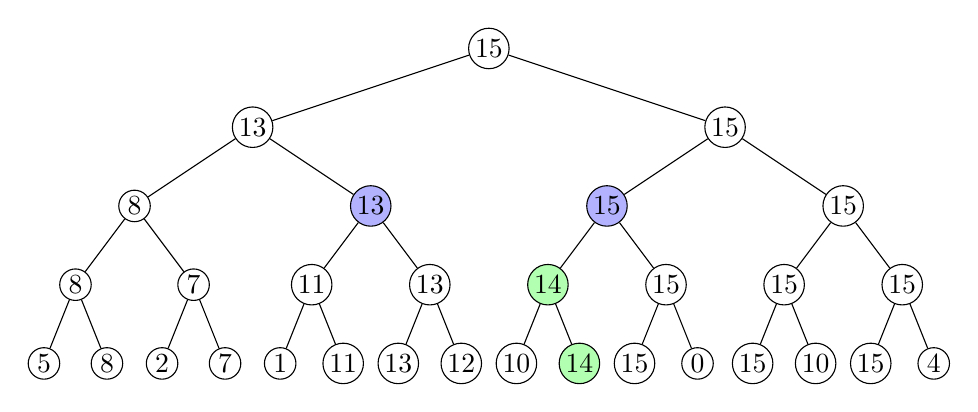
\begin{tikzpicture}[
        level distance=1cm,
        sibling distance=0pt,
        every node/.style = {circle, draw, minimum size=4mm, inner sep=1pt},
        level 1/.style={sibling distance=6cm},
        level 2/.style={sibling distance=3cm},
        level 3/.style={sibling distance=1.5cm},
        level 4/.style={sibling distance=0.8cm},
        level 5/.style={sibling distance=0.5cm}
      ]
      
      \node {15}
      child {node {13}
        child {node {8}
          child {node {8}
            child {node {5}}
            child {node {8}}
          }
          child {node {7}
            child {node {2}}
            child {node {7}}
          }
        }
        child {node[fill=blue!30] {13}
          child {node {11}
            child {node {1}}
            child {node {11}}
          }
          child {node {13}
            child {node {13}}
            child {node {12}}
          }
        }
      }
      child {node {15}
        child {node[fill=blue!30] {15}
          child {node[fill=green!30] {14}
            child {node {10}}
            child {node[fill=green!30] {14}}
          }
          child {node {15}
            child {node {15}}
            child {node {0}}
          }
        }
        child {node {15}
          child {node {15}
            child {node {15}}
            child {node {10}}
          }
          child {node {15}
            child {node {15}}
            child {node {4}}
          }
        }
      };
      
      \end{tikzpicture}
\end{center}

    \caption{The blue nodes are the ones that we performed binsearch on. The green nodes are the ones that binsearch traversed. The result of the query is index 10. As we can see, the first binsearch (on node with value 13 returned -1)}
    \label{fig:segment_tree_1}
\end{figure}

\section{Max prefix sum on Segment Tree}
In this section we will take look at a little bit more complex query which will require a little bit more complex segment tree.
Let's consider the following problem:
\begin{center}
    \textit{Given an array $a[1 \dots n]$, we want to be able to efficently answer a query $Q(i, j)$: What is the maximum prefix sum in subarray $a[i \dots j]$? 
    While still beeing able to perform point updates on array. }\\[1ex]
\end{center}

What structure we can use to solve this problem? ...You guessed it, segment tree! 
This time nodes of our segment tree will store more information than just a single value. 
We will store a pair of values in each node:
\begin{equation}
    (prefix, sum)
\end{equation}
Where \(prefix\) is the maximum prefix sum in the subtree of this node and \(sum\) is the sum of all elements in the subtree of this node. Before we construct the segment tree we need to define merge operation, that will be used to calculate the values in the parent node from the values in the child nodes.
\begin{algorithm}
    \caption{Merge Two Segments in Segment Tree}
    \begin{algorithmic}[1]
        \Procedure{Merge}{seg, index}
            \State $seg[index].sum \gets seg[2 * index].sum + seg[2 * index + 1].sum$
            \State $seg[index].prefix \gets 
                \max(seg[2 * index].prefix, seg[2 * index].sum + seg[2 * index + 1].prefix)$
        \EndProcedure
    \end{algorithmic}
\end{algorithm}


\begin{figure}[H]
    \centering
    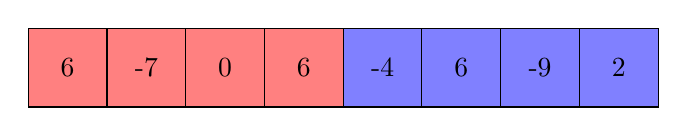
\begin{tikzpicture}
    % Define hardcoded values
    \def\values{6, -7, 0, 6, -4, 6, -9, 2}
    \foreach [count=\i from 0] \val in \values {
      \ifnum\i<4
        \definecolor{blockcolor}{rgb}{1,0.5,0.5} % light red
      \else
        \definecolor{blockcolor}{rgb}{0.5,0.5,1} % light blue
      \fi
  
      % Draw colored block
      \fill[blockcolor] (\i,0) rectangle ++(1,1);
      \draw (\i,0) rectangle ++(1,1);
      \node at (\i+0.5,0.5) {\val};
    }
  \end{tikzpicture}
  
    \caption{In this example the red blocks represent the subarray in left child and the blue blocks represent the subarray in right child. 
    Max predfix sum is ether the max prefix sum in left child or the sum of left child plus max prefix sum in right child. In this example the max prefix (equal to 7) of parent node is sum of left child plus max prefix of right child as it is greater than max prefix of left child (equal to 6).}
\end{figure}

Now we can construct the segment tree and perform point updates (left as excercise) exactly like in previos exmaples only this time we use the merge operation defined above.
Keeping in mind that when creating or updating the leaf node we need to set the prefix to the value of the element in the array.

Query operation on the other hand needs a little more modification.
We traverse the tree and find the nodes in the range just like in range query.
The result of the query is max prefix of some node plus sum of the nodes to the left we found during the traversal.
In particular the result might be max prefix of leftmost node in range or sum of all nodes we found.
\begin{figure}[H]
    \centering
    
\begin{center}
    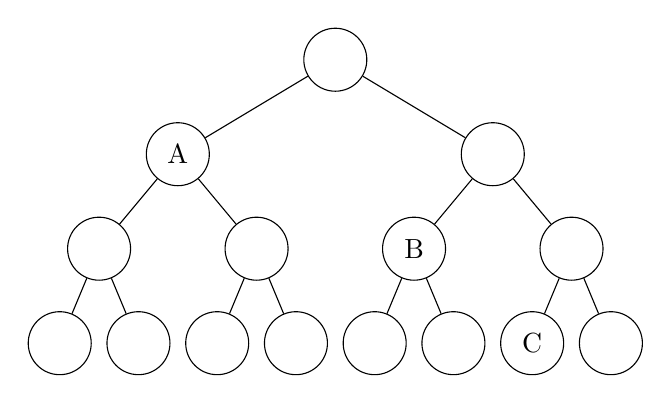
\begin{tikzpicture}[
      level distance=1.2cm,
      level 1/.style={sibling distance=4cm},
      level 2/.style={sibling distance=2cm},
      level 3/.style={sibling distance=1cm},
      every node/.style={draw,circle,minimum size=8mm,inner sep=1pt}
    ]
    
    % Root node with max value
    \node {}
        child {node {A}
            child {node {}
                child {node {}}
                child {node {}}
            }
            child {node {}
                child {node {}}
                child {node {}}
            }
        }
        child {node {}
            child {node {B}
                child {node {}}
                child {node {}}
            }
            child {node {}
                child {node {C}}
                child {node {}}
            }
        };
    
    \end{tikzpicture}
\end{center}
    \caption{Let $A,B,C$ be the nodes in the range of query. The result of this query would be $max(prefix(A), sum(A) + prefix(B), sum(A) + sum(B) + prefix(C))$.}
\end{figure}

Our range query, very similar to standard one, needs new variable $sum$, and a little modification 
when it finds a node in range:

\begin{algorithm}
    \caption{Range Max Prefix Query}
    \begin{algorithmic}[1]
        \Procedure{RangeQuery}{seg, index, l, r, a, b, sum}
            \Comment{sum: sum of all nodes in range to the left of current node}
            \If{$b \leq l$ \textbf{or} $r \leq a$}
                \State \Return $0$
            \ElsIf{$a \leq l$ \textbf{and} $r \leq b$}
                \State $tmp\_sum \gets sum$
                \State $sum += seg[index].sum$
                \State \Return $seg[index].prefix + tmp\_sum$ 
            \Else
                \State $mid \gets \left\lfloor \frac{l + r}{2} \right\rfloor$
                \State $left \gets$ \Call{RangeQuery}{seg, $2 \cdot index$, $l$, $mid$, $a$, $b$, $sum$}
                \State $right \gets$ \Call{RangeQuery}{seg, $2 \cdot index + 1$, $mid$, $r$, $a$, $b$, $sum$}
                \State \Return $\max(left, right)$
            \EndIf
        \EndProcedure
    \end{algorithmic}
\end{algorithm}

\section{Sweeping Line}
In this section we will use segment trees to implement a sweeping line algorithm.
Consider the following problem:
We are given a set of vertical and horizontal lines in a plane and we want to find the number of intersections between these lines.
The format of the input is as follows:
\begin{itemize}
    \item $n$ - number of lines
    \item $0 \leq x,y \leq 10^6$ - coordinates of the points that represent the lines.
    \item We can assume that the length of the line is greater than 0, we do not consider intersection at the endpoints of the lines and 2 parallel can't intersect.
    \item We are given number $n$ and $n$ touples $(x_1, y_1, x_2, y_2)$ where $(x_1, y_1)$ and $(x_2, y_2)$ are the coordinates of the endpoints of the line.
\end{itemize}

As we can see the problem is not online (we don't have to answer any queries) and yet the easiest way to solve it is to use a segmnet tree.
We perform something called a sweeping line algorithm. We will create from a segment tree a kind of brush that will sweep through the plane and count the intersections.
Lets say we swipe from left to right (we can do this from right to left or top to bottom as well). If our brush (we can also look at this as infinite vertical straight line) is at position $x$ we know that it stores all the lines that intersect this vertical line.
Knowing that we can ask how many lines intersect this vertical line at some range $(y1, y2)$, in anoter words for every vertical line at $x$ we know how many lines it intersects. How do we know that?
First of all we need to sort our input lines by their lower $x$ coordinate prioritizing the vertical lines.
Now we iterate over $x$ axis if we encounter the horizontal line we add 1 to the segment tree at position $y$ (the $y$ coordinate of the horizontal line).
If we encounter the end of the horizontal line we remove 1 from the segment tree at position $y$. You can see that the segment tree is used to store the number of horizontal lines
and the leaves of the tree represent the $y$ coordinates of the horizontal lines.
Now if we encounter a vertical line we can ask the segment tree how many horizontal lines intersect this vertical line at the range $(y1, y2)$. 
We add this number to the final result and continue iterating over the $x$ axis. 

\begin{figure}[H]
    \centering
    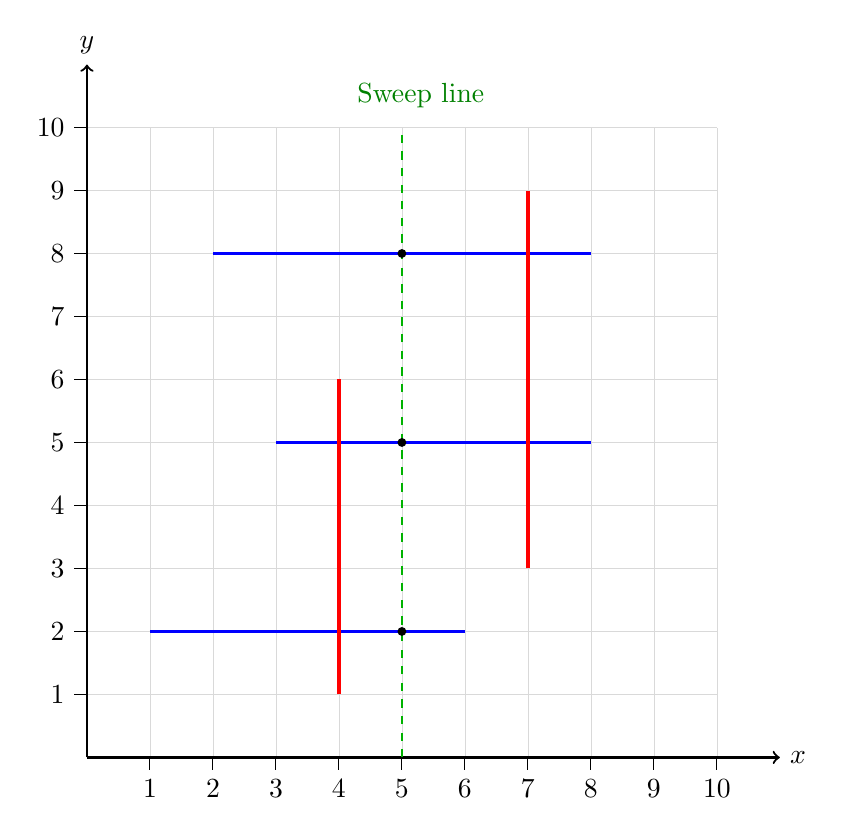
\begin{tikzpicture}[scale=0.8]
    \draw[step=1cm, gray!30, very thin] (0,0) grid (10,10);

    \draw[->, thick] (0,0) -- (11,0) node[right] {$x$};
    \draw[->, thick] (0,0) -- (0,11) node[above] {$y$};

    \foreach \x in {1,...,10}
        \draw (\x,0) -- (\x,-0.2) node[below] {\x};

    \foreach \y in {1,...,10}
        \draw (0,\y) -- (-0.2,\y) node[left] {\y};

    \draw[blue, very thick] (1,2) -- (6,2);
    \draw[blue, very thick] (3,5) -- (8,5);
    \draw[blue, very thick] (2,8) -- (8,8);

    \draw[red, very thick] (4,1) -- (4,6);
    \draw[red, very thick] (7,3) -- (7,9);

    \draw[green!70!black, thick, dashed] (5,0) -- (5,10);
    \node[green!50!black] at (5.3,10.5) {Sweep line};

    \fill[black] (5,2) circle (2pt);
    \fill[black] (5,5) circle (2pt);
    \fill[black] (5,8) circle (2pt);
\end{tikzpicture}
    \caption{This picture ilustrates algorithm in proces. The result so far is 2, intersections of the red line at $x=4$. Current state of segment trres leaves is $[0,0,1,0,0,1,0,0,1,0,0]$. }
\end{figure}

How does the operations on segment tree looks like then? 
This is acctually very simple segment tree with point update (add 1) and range query (sum on given range), which i described in the first section. The build operation is even simpler as we start with 0 in all leaves.

For easier implementation we store every line as node: \\
\textbf{Structure} \texttt{Line}  
\begin{itemize}
    \item \texttt{x1} : integer
    \item \texttt{y1} : integer
    \item \texttt{x2} : integer
    \item \texttt{y2} : integer
    \item \texttt{vertical} : boolean
\end{itemize}
The whole algorithm can be implemented as follows:

\begin{itemize}
    \item sort lines by x1 coordinate, if two lines have the same x1 choose the vertical line first
    \item initialize segment tree with size of $10^6$
    \item iterate over lines:
        \begin{itemize}
            \item if line is horizontal, add 1 to segment tree at position y1
            \item if line is vertical, query segment tree for range (y1, y2) and add result to final result
            \item if line is horizontal and we reached the end of the line, remove 1 from segment tree at position y2
        \end{itemize}
    \item return final result
\end{itemize}

Link to problem: \url{https://cses.fi/problemset/task/1740}

\end{document}